\documentclass[12pt]{article}
\usepackage{fixltx2e}
\title{Understanding transport in the H\textsubscript{II} Phase of Lyotropic Liquid Crystal Membranes}
\author{Benjamin J. Coscia\\
	Advisors: Michael Shirts, Richard Noble, Douglas Gin}
\usepackage[margin=1in]{geometry}
\usepackage{gensymb}
\usepackage{graphicx}
\usepackage{subcaption}
\usepackage{wrapfig}
\usepackage{cleveref}
\captionsetup{font=small}
\begin{document}
\bibliographystyle{ieeetran}
\maketitle
\section{Objective Statement}

Experimentalists lack a reliable procedure for identifying the best material for producing inverse hexagonal phase (H\textsubscript{II}) Lyotropic Liquid Crystal (LLC) membranes. Small angle X-ray scattering (SAXS) measurements confirm the hexagonal crystalline structure exhibited by the self-assembling liquid crystal (LC) monomers \cite{smith_ordered_1997}. TEM images support the hypothesis that the pores are aligned, straight, uniform in size and on the order of 1 nm in diameter \cite{feng_scalable_2014, feng_thin_2016}. Experiments tell us that the membrane selectively passes water while rejecting solutes on the order of 1 nm in diameter \cite{zhou_supported_2005}. Aside from heuristic arguments and fitting experimental data to constrained macroscopic models, we lack an understanding of why these membranes behave the way they do and consequently have no way of systematically improving them. All characterization and improvement has been done using a single starting monomer with, at most, minor variations to its structure. There are certainly other materials or derivatives which exhibit similar behavior with improved properties which is why there is a need for a reliable atomistic model that can explore a much wider chemical space. It is my goal to develop an accurate molecular model which accurately describes the microscopic structure and properties of H\textsubscript{II} LLC membranes. I will first develop a model based on the current membrane and experimental data and study it using Molecular Dynamics (MD) simulations. The procedure used in its development will then be generalized as a method for fast development of models of other potential H\textsubscript{II} forming LLC monomers. The flexibility of MD, efficient algorithms and mass computing power, will allow fast, relative to experiment, screening of large numbers of candidates. Viable candidates will be suggested to experimentalists for validation with an eventual feedback loop between experiment and modeling which will lead to optimized H\textsubscript{II} LLC membranes designed for a specific application.

\section{Significance}
H\textsubscript{II} LLC membranes were originally designed to see whether useful materials could be controllably synthesized at the nanometer scale \cite{smith_ordered_1997}. Their use has since been targeted as nanofiltration (NF) membranes for size selective filtration of molecules 1-10 nm in diameter \cite{zhou_supported_2005}. It is hypothesized that they can be used for desalination \cite{feng_scalable_2014} and general water treatment, such as cleaning up fracking water. Separation of solutes on the order of 1 nanometer in diameter during water treatment and desalination is a multi-faceted challenge requiring a process that is selective, high throughput and low energy \cite{daily_population_1992}. Membrane based processes have already been widely implemented in order to control water quality and composition. NF and reverse osmosis (RO) membranes are well suited for this purpose \cite{lee_review_2011, greenlee_reverse_2009, humplik_nanostructured_2011}. NF membrane have pore sizes on the order of 1 nm in size which separates solutes on the basis of size exclusion and, in the case of polarizable or charged solutes, electrostatic repulsions  \cite{humplik_nanostructured_2011}. RO separates based on the relative solubilities and diffusivities of solutes in the membrane’s dense polymer matrix \cite{wijmans_solution-diffusion_1995}. Despite the difference in the mechanism of solute transport in each type of membrane, the flux of solute through the membrane can be shown to be proportional to the applied pressure and inversely proportional to the membrane thickness \cite{wijmans_solution-diffusion_1995}. Hence, maximum throughput can be achieved by increasing the applied pressure and by making very thin membranes. Unfortunately, controlling membrane architecture is near impossible using conventional polymer membrane synthetic techniques. NF membranes typically have tortuous pores, increasing the effective membrane thickness, with a distribution of pore radii, limiting selectivity \cite{lau_recent_2012}. Since RO membranes rely on the diffusive motion of solutes through the polymer matrix, the path followed by solutes is tortuous. The membrane’s density also requires much higher applied pressures driving up energy costs. Materials used for RO are limited as well since they must be chosen based on its interaction with desired separation solute \cite{fritzmann_state---art_2007}.

H\textsubscript{II} LLC membranes have straight, uniform, nanometer scale pores which can give optimal throughput given a sufficiently thin membrane. Additionally, the chemistry of the LC monomer used to assemble the membrane can be changed \cite{zhou_supported_2005} presumably leading to different solute rejecting properties. They can be tailored to specific applications including not only nanofiltration and desalination, but gas separations and as selective vapor barriers \cite{gin_polymerized_2008}, and even as templates for catalytic particles and functional groups \cite{ding_catalytic_2000}. The culmination of this remains to be seen through modeling and experimentation, but the impact of this technology working as hypothesized can lead to a revolution in membrane technology.

\section{Background and Literature Review}
Nanostructured membrane materials are particularly promising because they offer nanoscale control \cite{humplik_nanostructured_2011}. Solute rejecting pores can be tuned to appropriate sizes for size exclusion filtration, functional groups can be added to enhance selectivity, and pore shape and size are well-defined which all facilitate better performance and performance prediction.

Nanostructured materials are not without limitations. Leading nanostructured filtration technologies include graphene sheets, carbon nanotubes (CNTs), and metal organic frameworks (MOFs). Graphene sheets are atomically thick which gives excellent permeability, but in practice, defects are easily introduced during manufacturing which severely decreases performance \cite{cohen-tanugi_multilayer_2016}. Molecular dynamic studies of carbon nanotube embedded membranes have shown their ability to completely reject solutes. Developing synthetic methods to achieve the same pore uniformity and alignment that was simulated is a significant challenge for implementation beyond the lab scale \cite{mauter_environmental_2008}. MOFs are a successful nanostructured technology particularly for gas separation applications because of their ability to selectively adsorb gases such as CH\textsubscript{4} and H\textsubscript{2}. Unfortunately, they are unstable in water making them ineffective nanofiltration membranes \cite{dias_towards-2015}. 

Lyotropic Liquid Crystals (LLCs) offer the opportunity to create highly ordered membrane structures with tunable properties for a variety of applications including desalination and wastewater treatment. This class of organic compounds forms a range of crystalline phases including lamellar, bicontinuous cubic and hexagonal phases based on monomer structure and initial solution composition \cite{lee_polymerization_1995, smith_ordered_1997}.

The structure of the LLC materials has the potential to address demands in wastewater treatment and desalination. In the presence of c.a. 10 \% water, the monomer to be studied in this paper, shown in figure 1, forms the H\textsubscript{II} phase consisting of vertically aligned nanopores of uniform size, packed in a hexagonal array \cite{smith_ordered_1997,resel_structural_2000}. In the absence of water a thermotropic columnar phase, termed Col\textsubscript{h}, self assembles into the same hexagonal morphology, absent of water, and is stable up to its isotropic transition point at 65.6 \degree C. Hydrophilic regions of monomer are oriented inward forming aqueous pores. Until recently, this type of behavior was only seen in mesoscopic domains with no macroscopic pore alignment which prevented competitive fluxes\cite{zhou_supported_2005}. Feng et al. has since been able to manipulate the material into membrane sheets with uniform alignment using electromagnetic alignment and soft confinement techniques, followed by a free radical crosslinking reaction used to maintain the film’s structure\cite{feng_scalable_2014,feng_thin_2016}. With this advance, further experimental work is being done to characterize LLC membranes. Nearly straight pores combined with Donnan exclusion and molecular sieving promise a future LLC H\textsubscript{II} phase membrane offering high permeability and selectivity with subsequent low energy consumption.
\begin{figure}
\centering
	\begin{subfigure}{.3\textwidth}
		\centering
		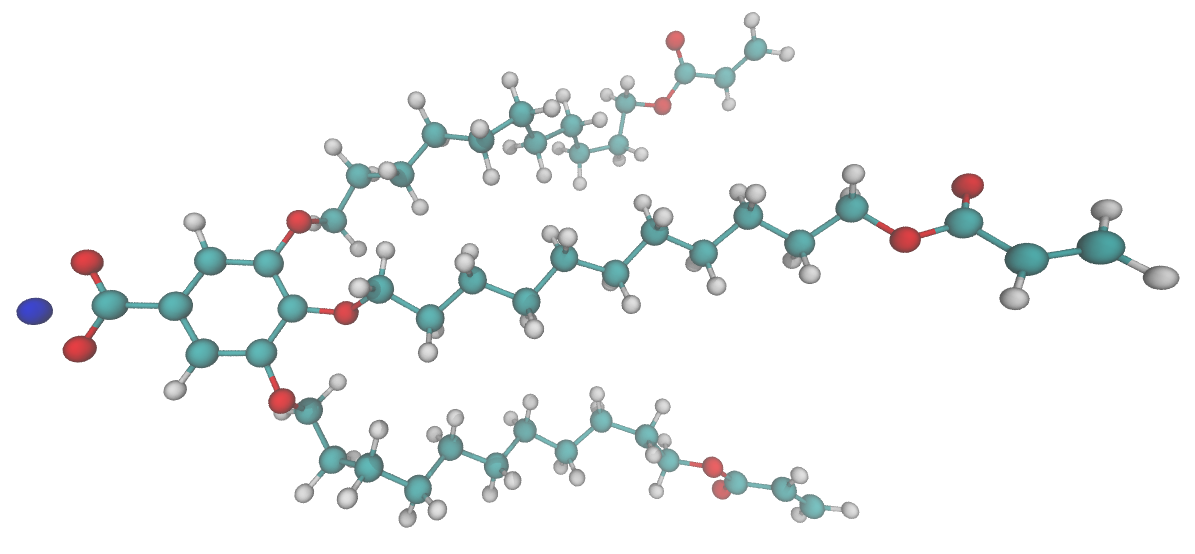
\includegraphics[width=\linewidth]{monomer.png}
		\label{fig:monomer}
		\caption{}
	\end{subfigure}
	\begin{subfigure}{.3\textwidth}
		\centering % material in its scope will be centered
		\includegraphics[width=\linewidth]{Top_View_4_3.png}
		\label{fig:TopView}
		\caption{}
	\end{subfigure}
	\begin{subfigure}{.3\textwidth}
		\centering
		\includegraphics[width=\linewidth]{Side_Profile.png}
		\label{fig:SideProfile}
		\caption{}
	\end{subfigure}
	\caption{(a) Monomer Na-GA3C11 (b) Top View of hexagonally packed system made with Na-GA3C11. Sodium ions are colored blue. Red lines are vinyl groups from each tail of the monomer (c) Side Profile of hexagonally packed system. Sodium ions are emphasized in blue to show that the pores run straight through the membrane}
	\label{fig:System}
\end{figure}
Modeling LLC systems, in particular the H\textsubscript{II}  and Col\textsubscript{h} phases, is new to the field, however we can draw on work done on similar systems from other fields in order to inform our own work. Biological ion channels have long been studied using MD simulations. Ion channels are embedded into cell membranes and gate ion passage into cells inducing a membrane potential and regulating cell volume. Methods used to measure ion conduction in ion channels are being adapted to the LLC system for direct comparison to experiment. \cite{aksimentiev_imaging_2005, gumbart_constant_2012}. CNTs have been extensively studied with MD and exhibit fast water conduction through the membrane pores. Techniques used to study the mechanism of water and solute transport in CNTs are necessary to understand transport mechanisms in LLCs \cite{zhu_water_2003}.

\section{Methods}

H\textsubscript{II} monomers were parameterized using the Generalized Amber Forcefield (GAFF) with the Antechamber package provided with AmberTools16\cite{case_ambertools16_2016,wang_development_2004, wang_automatic_2006}. All molecular dynamics simulations are run using Gromacs 5.1.2 and later versions as they are released \cite{bekker_gromacs:_1993, berendsen_gromacs:_1995, lindahl_gromacs_2001, van_der_spoel_gromacs:_2005, hess_gromacs_2008}. Long, computationally intensive simulations are run using the HPC resources Janus and Bridges \cite{nystrom_bridges:_2015, towns_xsede:_2014}.

An assembly code was written in python to place parameterized and energy minimized monomers into the expected cylindrical form (Figure \ref{fig:TopInit}). A monoclinic unit cell was chosen since it is the smallest unit cell which will still form a hexagonal packing. Four pores consisting of stacked rings of monomer were placed inside the unit cell with hydrophilic head groups oriented towards the center of the pore. Number of layers, number of monomers per layer, pore radius, distance between pore centers, and distance between layers are all adjustable parameters along with the monomer chosen to build the structure.

\begin{wrapfigure}{R}{0.3\textwidth}
	\centering
	\includegraphics[width=0.3\textwidth]{Top_Init.png}
	\caption{\label{fig:TopInit} A top down view of the initial configuration created using the assembly python script}
\end{wrapfigure}

Although in the limit of infinite time, the system will settle into its lowest energy configuration, the H\textsubscript{II} phase, the length of time for the system to reach that state varies with choice of starting conditions. To equilibrate fastest, and avoid entrapment in metastable states, choice of initial configuration dimensions are best chosen according to developed guidelines (available upon request).

Following creation of an initial structure, simulations are run at 300 K and 1 bar (The NPT ensemble). From a visual perspective, the pores stay packed in a hexagonal configuration (See Figure \ref{fig:System}b). To address subtleties which the eye cannot see, a set of tools were coded to monitor system equilibration. One of the most useful tools quantifies the ‘hexagonality’ of the system. To do so, the x and y coordinates of the sodium of ions in each pore were averaged and treated as a central axis running straight down in each pore. The distance between these axes were used to quantify the hexagonal character of the system. In a perfectly hexagonal system, all pore-to-pore distances would be equal. To achieve this character, simulations greater than 100 ns were necessary.

After equilibration, the system is solvated with water then simulated further to allow water molecules to naturally penetrate the hydrophilic pores. Alternatively, one can skip the water solvation step to study the thermotropic Col\textsubscript{h} system. Whichever route is chosen, it is necessary to follow equilibration with a crosslinking reaction. Macroscopically this is an important step in order to maintain long range pore alignment. Microscopically it is important as a way to make sure we are modeling the exact system. It also locks in the equilibrium structure and eliminates any worries about fluctuations away from it.
 
A generic crosslinking algorithm is not available and thus required the creation of my own based on my knowledge of the crosslink reaction and work done by other authors on similar systems \cite{jang_relative_2012}. The crosslinking reaction is a free radical polymerization of terminal vinyl groups on each of the three monomer tails. On a high level, the algorithm calculates distances between potentially bonding carbons after a short simulation. Carbons meeting a distance cutoff criteria are bonded together or terminated with a specified probability. Carbons that would be left as radicals are flagged as a way to increase reactivity on future iterations. The process is repeated until reasonable bonds between eligible carbons can no longer be made. 

The careful development of this methodology will make it applicable to other LLC systems.

\section{Progress to Date}

(‘lots’ of pictures in this section)
The first phase of this project has been defined by the development of an accurate membrane model. To date, that goal is nearly achieved. The system has yet to be fully solvated but there is experimental data of the thermotropic Colh phase which parallels that of the H\textsubscript{II} phase and can be used in the development of the model. Using this experimental data as a benchmark, we have created an LLC system that equilibrates to a geometry consistent with TEM and SAXS data. (Figure). The spacing between pores is 4.14 +/- 0.05 nm. The radius of the pores, as defined by the ring of highest sodium density, are 1.2 nm. Also, a reliable crosslinking procedure has been implemented which can lock in the equilibrium structure of the membrane and match the real system.
The last step in model validation requires that the model accurately predicts experimental conductivity measurements. In the process, I will develop a general method for measuring conductivity based on MD output. To date, I have identified three possible routes for making these predictions. The Nernst Einstein relation is the simplest and is based on ion diffusivity… Fluctation-dissipation theorem … CompEL type technique. 
In parallel, I have learned how to best utilize the HPC resources available by conducting scaling studies on each resources. I have learned how and developed methods to optimally parallelize Gromacs simulations on Janus and Bridges using both MPI and GPUs. This will allow us to run more simulations in a shorter amount which will be instrumental to high throughput screening.  

\section{Research Plan}

My immediate goals, which I hope to complete by my first thesis committee meeting are to have developed a fully validated molecular model of H\textsubscript{II} LLC systems. Beyond just matching experimental data, I would like learn more about the structure that experiments cannot tell us. A major question of interest to me is understanding how many monomer are in each disk that make up the membrane pores. As it stands, it is unclear whether there are 5, 6, 7 or some combination of these amounts stacked in alternating layers. I will assemble reasonable structures and conduct free energy calculations to make clear which ensemble the membrane system is most stable in. This is a computationally expensive task that may prove necessary if we see inconsistent property predictions between models made up of different compositions. Additionally, I plan to understand the mechanism of solute transport for a few select molecules. I am particularly interested in the transport of sodium chloride as I’d like to see this membrane applied as a desalination technology.
My long term goals are to use the model to direct membrane design in the Gin and Noble labs. I plan to create an organized and versatile python package which can be used to design LLC membranes for separation of small molecules of choice. If possible, I’d like to develop my own macroscopic model which can be used to predict structures without the computational expensive of MD simulations. I plan to get in the lab myself and get to work designing these advanced materials. Ultimately I hope to make the design of LLC membranes more systematic and fast.

\bibliography{Prelim}

\end{document}